% -*- Mode:TeX -*-

%% IMPORTANT: The official thesis specifications are available at:
%%            http://libraries.mit.edu/archives/thesis-specs/
%%
%%            Please verify your thesis' formatting and copyright
%%            assignment before submission.  If you notice any
%%            discrepancies between these templates and the 
%%            MIT Libraries' specs, please let us know
%%            by e-mailing thesis@mit.edu

%% The documentclass options along with the pagestyle can be used to generate
%% a technical report, a draft copy, or a regular thesis.  You may need to
%% re-specify the pagestyle after you \include  cover.tex.  For more
%% information, see the first few lines of mitthesis.cls. 

%\documentclass[12pt,vi,twoside]{mitthesis}
%%
%%  If you want your thesis copyright to you instead of MIT, use the
%%  ``vi'' option, as above.
%%
%\documentclass[12pt,twoside,leftblank]{mitthesis}
%%
%% If you want blank pages before new chapters to be labelled ``This
%% Page Intentionally Left Blank'', use the ``leftblank'' option, as
%% above. 

\documentclass[12pt,twoside]{mitthesis}
\usepackage{lgrind}
%% These have been added at the request of the MIT Libraries, because
%% some PDF conversions mess up the ligatures.  -LB, 1/22/2014
\usepackage{cmap}
\usepackage{amsmath}
\usepackage[T1]{fontenc}

% Added by me - makes the TOC into hyperlinks
\usepackage{color}
\usepackage{hyperref}
\hypersetup{
    colorlinks,
    citecolor=blue,
    filecolor=black,
    linkcolor=blue,
    urlcolor=blue
}

\pagestyle{plain}


%% This bit allows you to either specify only the files which you wish to
%% process, or `all' to process all files which you \include.
%% Krishna Sethuraman (1990).

\begin{document}

% -*-latex-*-
% 
% For questions, comments, concerns or complaints:
% thesis@mit.edu
% 
%
% $Log: cover.tex,v $
% Revision 1.8  2008/05/13 15:02:15  jdreed
% Degree month is June, not May.  Added note about prevdegrees.
% Arthur Smith's title updated
%
% Revision 1.7  2001/02/08 18:53:16  boojum
% changed some \newpages to \cleardoublepages
%
% Revision 1.6  1999/10/21 14:49:31  boojum
% changed comment referring to documentstyle
%
% Revision 1.5  1999/10/21 14:39:04  boojum
% *** empty log message ***
%
% Revision 1.4  1997/04/18  17:54:10  othomas
% added page numbers on abstract and cover, and made 1 abstract
% page the default rather than 2.  (anne hunter tells me this
% is the new institute standard.)
%
% Revision 1.4  1997/04/18  17:54:10  othomas
% added page numbers on abstract and cover, and made 1 abstract
% page the default rather than 2.  (anne hunter tells me this
% is the new institute standard.)
%
% Revision 1.3  93/05/17  17:06:29  starflt
% Added acknowledgements section (suggested by tompalka)
% 
% Revision 1.2  92/04/22  13:13:13  epeisach
% Fixes for 1991 course 6 requirements
% Phrase "and to grant others the right to do so" has been added to 
% permission clause
% Second copy of abstract is not counted as separate pages so numbering works
% out
% 
% Revision 1.1  92/04/22  13:08:20  epeisach

% NOTE:
% These templates make an effort to conform to the MIT Thesis specifications,
% however the specifications can change.  We recommend that you verify the
% layout of your title page with your thesis advisor and/or the MIT 
% Libraries before printing your final copy.
\title{An Optimizing Compiler for Low-Level Floating Point Operations}

\author{Lucien William Van Elsen}
% If you wish to list your previous degrees on the cover page, use the 
% previous degrees command:
%       \prevdegrees{A.A., Harvard University (1985)}
% You can use the \\ command to list multiple previous degrees
%       \prevdegrees{B.S., University of California (1978) \\
%                    S.M., Massachusetts Institute of Technology (1981)}
\department{Department of Electrical Engineering and Computer Science}

% If the thesis is for two degrees simultaneously, list them both
% separated by \and like this:
% \degree{Doctor of Philosophy \and Master of Science}
\degree{Bachelor of Science in Computer Science and Engineering}

% As of the 2007-08 academic year, valid degree months are September, 
% February, or June.  The default is June.
\degreemonth{June}
\degreeyear{1990}
\thesisdate{May 18, 1990}

%% By default, the thesis will be copyrighted to MIT.  If you need to copyright
%% the thesis to yourself, just specify the `vi' documentclass option.  If for
%% some reason you want to exactly specify the copyright notice text, you can
%% use the \copyrightnoticetext command.  
%\copyrightnoticetext{\copyright IBM, 1990.  Do not open till Xmas.}

% If there is more than one supervisor, use the \supervisor command
% once for each.
\supervisor{William J. Dally}{Associate Professor}

% This is the department committee chairman, not the thesis committee
% chairman.  You should replace this with your Department's Committee
% Chairman.
\chairman{Arthur C. Smith}{Chairman, Department Committee on Graduate Theses}

% Make the titlepage based on the above information.  If you need
% something special and can't use the standard form, you can specify
% the exact text of the titlepage yourself.  Put it in a titlepage
% environment and leave blank lines where you want vertical space.
% The spaces will be adjusted to fill the entire page.  The dotted
% lines for the signatures are made with the \signature command.
\maketitle

% The abstractpage environment sets up everything on the page except
% the text itself.  The title and other header material are put at the
% top of the page, and the supervisors are listed at the bottom.  A
% new page is begun both before and after.  Of course, an abstract may
% be more than one page itself.  If you need more control over the
% format of the page, you can use the abstract environment, which puts
% the word "Abstract" at the beginning and single spaces its text.

%% You can either \input (*not* \include) your abstract file, or you can put
%% the text of the abstract directly between the \begin{abstractpage} and
%% \end{abstractpage} commands.

% First copy: start a new page, and save the page number.
\cleardoublepage
% Uncomment the next line if you do NOT want a page number on your
% abstract and acknowledgments pages.
% \pagestyle{empty}
\setcounter{savepage}{\thepage}
\begin{abstractpage}
% $Log: abstract.tex,v $
% Revision 1.1  93/05/14  14:56:25  starflt
% Initial revision
% 
% Revision 1.1  90/05/04  10:41:01  lwvanels
% Initial revision
% 
%
%% The text of your abstract and nothing else (other than comments) goes here.
%% It will be single-spaced and the rest of the text that is supposed to go on
%% the abstract page will be generated by the abstractpage environment.  This
%% file should be \input (not \include 'd) from cover.tex.
In this thesis, I designed and implemented a compiler which performs
optimizations that reduce the number of low-level floating point operations
necessary for a specific task; this involves the optimization of chains of
floating point operations as well as the implementation of a ``fixed'' point
data type that allows some floating point operations to simulated with integer
arithmetic.  The source language of the compiler is a subset of C, and the
destination language is assembly language for a micro-floating point CPU.  An
instruction-level simulator of the CPU was written to allow testing of the
code.  A series of test pieces of codes was compiled, both with and without
optimization, to determine how effective these optimizations were.

\end{abstractpage}

% Additional copy: start a new page, and reset the page number.  This way,
% the second copy of the abstract is not counted as separate pages.
% Uncomment the next 6 lines if you need two copies of the abstract
% page.
% \setcounter{page}{\thesavepage}
% \begin{abstractpage}
% % $Log: abstract.tex,v $
% Revision 1.1  93/05/14  14:56:25  starflt
% Initial revision
% 
% Revision 1.1  90/05/04  10:41:01  lwvanels
% Initial revision
% 
%
%% The text of your abstract and nothing else (other than comments) goes here.
%% It will be single-spaced and the rest of the text that is supposed to go on
%% the abstract page will be generated by the abstractpage environment.  This
%% file should be \input (not \include 'd) from cover.tex.
In this thesis, I designed and implemented a compiler which performs
optimizations that reduce the number of low-level floating point operations
necessary for a specific task; this involves the optimization of chains of
floating point operations as well as the implementation of a ``fixed'' point
data type that allows some floating point operations to simulated with integer
arithmetic.  The source language of the compiler is a subset of C, and the
destination language is assembly language for a micro-floating point CPU.  An
instruction-level simulator of the CPU was written to allow testing of the
code.  A series of test pieces of codes was compiled, both with and without
optimization, to determine how effective these optimizations were.

% \end{abstractpage}

\cleardoublepage

\section*{Acknowledgments}

This is the acknowledgements section.  You should replace this with your
own acknowledgements.

%%%%%%%%%%%%%%%%%%%%%%%%%%%%%%%%%%%%%%%%%%%%%%%%%%%%%%%%%%%%%%%%%%%%%%
% -*-latex-*-

% Some departments (e.g. 5) require an additional signature page.  See
% signature.tex for more information and uncomment the following line if
% applicable.
% % -*- Mode:TeX -*-
%
% Some departments (e.g. Chemistry) require an additional cover page
% with signatures of the thesis committee.  Please check with your
% thesis advisor or other appropriate person to determine if such a 
% page is required for your thesis.  
%
% If you choose not to use the "titlepage" environment, a \newpage
% commands, and several \vspace{\fill} commands may be necessary to
% achieve the required spacing.  The \signature command is defined in
% the "mitthesis" class
%
% The following sample appears courtesy of Ben Kaduk <kaduk@mit.edu> and
% was used in his June 2012 doctoral thesis in Chemistry. 

\begin{titlepage}
\begin{large}
This doctoral thesis has been examined by a Committee of the Department
of Chemistry as follows:

\signature{Professor Jianshu Cao}{Chairman, Thesis Committee \\
   Professor of Chemistry}

\signature{Professor Troy Van Voorhis}{Thesis Supervisor \\
   Associate Professor of Chemistry}

\signature{Professor Robert W. Field}{Member, Thesis Committee \\
   Haslam and Dewey Professor of Chemistry}
\end{large}
\end{titlepage}


\pagestyle{plain}
  % -*- Mode:TeX -*-
%% This file simply contains the commands that actually generate the table of
%% contents and lists of figures and tables.  You can omit any or all of
%% these files by simply taking out the appropriate command.  For more
%% information on these files, see appendix C.3.3 of the LaTeX manual. 
\tableofcontents
\addcontentsline{toc}{chapter}{Symbols}
\newpage
\listoffigures
\newpage
\listoftables


%% This is an example first chapter.  You should put chapter/appendix that you
%% write into a separate file, and add a line \include{yourfilename} to
%% main.tex, where `yourfilename.tex' is the name of the chapter/appendix file.
%% You can process specific files by typing their names in at the 
%% \files=
%% prompt when you run the file main.tex through LaTeX.

\glsxtrnewsymbol[
 description={vector of states, pre-correction}]{x-}{\ensuremath{\mathbf{x^{-}}}}
\glsxtrnewsymbol[description={vector of states, post-correction}]{x+}{\ensuremath{\mathbf{x^{+}}}}
\glsxtrnewsymbol[description={vector of predicted states}]{y}{\ensuremath{\mathbf{y}}}
\glsxtrnewsymbol[description={vector of parameters, pre-correction}]{theta-}{\ensuremath{\mathbf{\theta^{-}}}}
\glsxtrnewsymbol[description={vector of parameters, post-correction}]{theta+}{\ensuremath{\mathbf{\theta^{+}}}}
\glsxtrnewsymbol[description={A vector of size $\theta$ sampled from the grand mean and grand standard deviation of all members of $\theta$ across all ensembles of $\theta$}]{Upsilon}{\ensuremath{\Upsilon}}
\glsxtrnewsymbol[description={A vector of theta taken from the grand mean and grand standard deviation of all thetas across all ensembles}]{Upsilon}{\ensuremath{\Upsilon}}
\glsxtrnewsymbol[description={vector of forcing data}]{u}{\ensuremath{\mathbf{u}}}
\glsxtrnewsymbol[description={vector of observed states}]{z}{\ensuremath{\mathbf{z}}}
\glsxtrnewsymbol[description={ensemble member}]{i}{\ensuremath{i}}
\glsxtrnewsymbol[description={timestep}]{t}{\ensuremath{t}}
\glsxtrnewsymbol[description={vector of error: model uncertainty}]{epsilon}{\ensuremath{\varepsilon}}
\glsxtrnewsymbol[description={vector of error: observed uncertainty}]{delta}{\ensuremath{\delta}}
\glsxtrnewsymbol[description={forcing data error covariance matrix}]{Q}{\ensuremath{Q}}
\glsxtrnewsymbol[description={observation error covariance matrix}]{R}{\ensuremath{R}}
\glsxtrnewsymbol[description={Kernel smoothing mixing parameter}]{a}{\ensuremath{a}}
\glsxtrnewsymbol[description={Hierarchical parameter perturbation mixing parameter vector}]{alpha}{\ensuremath{\alpha}}
\glsxtrnewsymbol[description={Hierarchical parameter perturbation mixing parameter}]{b}{\ensuremath{b}}
\glsxtrnewsymbol[description={Hierarchical group}]{g}{\ensuremath{g}}
\glsxtrnewsymbol[description={Set of vectors in hierarchical group $g$}]{G}{\ensuremath{G_{g}}}
\glsxtrnewsymbol[description={Model function}]{ffunc}{\ensuremath{f()}}
\glsxtrnewsymbol[description={Masking function (allows comparison of observations and matching states)}]{hfunc}{\ensuremath{h()}}
\glsxtrnewsymbol[description={Kalman gain matrix}]{K}{\ensuremath{K}}
\glsxtrnewsymbol[description={Shorthand for covariance}]{Sigma}{\ensuremath{\Sigma}}
\chapter{Introduction}



	Utilizing sequential data assimilation techniques to filter hydrologic models is an efficient way to correct and calibrate them both before and after implementation in the field. Many observations such as SWE, streamflow, and precipitation are collected on a daily basis across various geographic regions, allowing the previous day's information to be dynamically ingested by the hydrologic model and inform current predictions. These models allow hydrologists to understand the past and predict the future.
	
	Models that ingest data sequentially can be efficiently corrected by a Kalman Filter, a sequential data assimilation algorithm. Kalman Filters only need the previous timestep's state estimate, parameter estimate, and co-variance matrices to update the current timestep's state estimate, parameter estimate, and co-variance matrices. However, the original Kalman filter\cite{Kalman1960} was created to solve linear problems, and more complicated implementations must be used to solve non-linear problems. The extended Kalman Filter\cite{Jazwinski1970} works for mildly non-linear systems but does not function optimally on heavily non-linear systems\cite{Miller1994}. The Unscented Kalman Filter\cite{Julier1997} is an all-around improvement on the Extended Kalman Filter that allows for the filtering of highly non-linear systems. The Ensemble Kalman Filter\cite{Evensen1994}, a predecessor to the Unscented Kalman Filter, filters non-linear systems by generating an 'ensemble' of model instances and adding unique noise to each model's forcing data. The main advantage of this ensemble based approach is the substitution of the original Kalman Filter's error covarience matrix with an ensemble covariance matrix, which allows for the efficient computation of the covariance of high dimensional state vectors. 
	
	In order to calibrate parameters within a hydrologic model a Dual State Kalman Filter may be used. Dual state Kalman filters add a small perturbation to a series of parameters that the use rwishes to calibrate. These perturbed parameters vectors are then corrected in a similar fashion to the state vectors. After this happens a 'second' filter runs and corrects the state vectors in the normal fashion. The Dual State Ensemble Kalman Filter implemented by Moradkhani et. al\cite{Moradkhani2005} extends the Ensemble Kalman Filter into a dual state configuration.
	
	 To examines the Dual State Ensemble Kalman Filter's application to high dimensional geospatially distributed raster data Professor Marko Maneta's \textbf{daWUAPhydroengine} is used. Professor Maneta and his team have created a hydrological rainfall-runoff model that predicts streamflows across the state of Montana. \textbf{daWUAPhydroengine} is informed by a variety of smaller models, including a groundwater model, snow water equivalient (swe) model, and agricultural component model. Despite this complexity, \textbf{daWUAPhydroengine} is designed to be a quick and efficient model. \textbf{daWUAPhydroengine} is influenced by a series of uncalibrated high-dimensional parameters that are stored as 2D raster data. A Dual Ensemble Kalman Filter is an optimal calibration algorithm to calibrate this raster data because 1) the DEnKF does not have to compute the high dimensional state covariance matrix and 2) \textbf{daWUAPhydroengine} is a sequential model.
	
	Chapter 2 covers the methods behind the Dual Ensemble Kalman Filtering algorithm originally implemented by Moradkhani et al. Chapter 3 displays results of applying the Dual State Kalman Filter to \textbf{daWUAPhydroengine}. Chapter 4 discusses improvements currently being made, particularly the plans for a new, innovative hierarchical algorithm.
	
	
	

	
\chapter{Introduction}



	Utilizing sequential data assimilation techniques to filter the output of hydrologic models is an efficient way to correct and calibrate hydrologic models before and after their implementation in scientific studies or public projects \cite{Reichle2002}, \cite{Moradkhani2005}, \cite{Reichle2008}. Observations such as SWE (snow water equivalent), streamflow, and precipitation are collected on a daily basis across various geographic regions, allowing  real time information to be dynamically ingested by the hydrologic model and inform present and future predictions. More accurate models allow hydrologists to better understand the past and predict the future, and the need to research optimal methods of hydrologic data assimilation has been recognized \cite{Troch2003} and researched \cite{Liu2007}, \cite{Reichle2008}. Observed hydrologic data may allow models that output streamflow or SWE states, such as rainfall-runoff models, to undergo parameter estimation. Many empirical parameters exist in hydrologic models such as the HBV model to account for wildcard environmental attributes such as the temperature threshold for melting snow in a snowpack system \cite{Maneta2008}, the percolation of water from the upper to the lower reservoir of a groundwater system \cite{Maneta2008}, or the dispersion of a wave through a channel in a Muskingham-Cunge routing system \cite{Montero2016}. These parameters are frequently correlated and can have more then one set of values that produce good results \cite{Jakeman1993}, \cite{Maneta2008}. Parameter estimation for rainfall-runoff models has been an active area of research \cite{Sorooshian1980},\cite{Sorooshian1993} and research has progressed into the 21'st century \cite{Moradkhani2005}, \cite{Wagener2006}, \cite{Reichle2008}.
	
	Models that ingest data sequentially can have their variables efficiently filtered by a Kalman Filter, a sequential data assimilation algorithm. Kalman Filters only need the previous timestep's state estimate and covariance matrices to update the current timestep's state estimate and covariance matrices based on a new observed state. The original Kalman filter\cite{Kalman1960} was created to solve linear problems and more complicated implementations must be used to solve non-linear problems. The extended Kalman Filter\cite{Jazwinski1970} works for mildly non-linear systems but does not function optimally on strongly non-linear systems\cite{Miller1994}. The Unscented Kalman Filter\cite{Julier1997} is an improvement on the Extended Kalman Filter that allows for the filtering of highly non-linear systems. The Ensemble Kalman Filter\cite{Evensen1994}, a predecessor to the Unscented Kalman Filter, filters non-linear systems by generating an 'ensemble' of model instances and adding unique noise to each instance's forcing data. The main advantage of this ensemble based approach is the EnKF's capacity to approximate the complete prosterior of a problem as opposed to the Bayesian approximation calculated through the Unscented Kalman Filter method.  The substitution of the original Kalman Filter's error covarience matrix with an ensemble covariance matrix also allows for the efficient computation of the covariance of high dimensional state vectors.
	
	To calibrate model parameters as well as model states a Dual State Kalman Filter may be used as demonstrated by Moradkhani et. al in 2005 \cite{Moradkhani2005}. Dual state Kalman filters add a small perturbation to a series of parameters that the user wishes to calibrate. These perturbed parameters vectors are then corrected in a similar fashion to the state vectors. After this happens a second filter is run to correct the state vectors in the traditional fashion. The Dual State Ensemble Kalman Filter implemented by Moradkhani et. al\cite{Moradkhani2005} extends the Ensemble Kalman Filter into a dual state configuration and is shown to successfully predict a set of parameters.
	
	An alternative method of parameter estimation that utilizes the Kalman Filter is the Joint Kalman Filter, which combines states and parameters into one vector that is calculated simultaneously without the need for a second run. Joint Ensemble Kalman Filters have been successfully implemented on hydrologic models \cite{Vrugt2005}, \cite{Xiong2019} and other models \cite{Chen2008}, but Joint Ensemble Kalman filters can suffer from "filter inbreeding" under certain circumstances \cite{HendricksFranssen2008} and introduce inconsistency in especially heterogeneous formations \cite{Wen2006}. Overall Dual Ensemble Kalman Filters have been shown to produce more accurate parameter estimations then Joint Ensemble Kalman Filters, especially in noisy situations or non-linear environments, with the major drawback of the Dual approach being its larger draw on computational power \cite{Mariani2005}.
	
	In this paper hierarchical modeling techniques are integrated into the Dual State Ensemble Kalman Filter's parameter perturbation equation to create a Hierarchical Dual State Ensemble Kalman Filter. A hierarchical parameter perturbation framework allows the model to account for parameters that are potentially hierarchically related. For example, the celerity being calculated for a series of subbasins may be hierarchically related to each other because of a larger watershed or geological feature enveloping them. To examine the Dual State Hierarchical Ensemble Kalman Filter's application to high dimensional spatially distributed raster data and geographical data the hydrologic model, a variation of a rainfall-runoff model, is implemented to predict streamflows across the state of Montana. The hydrologic model is informed by a variety of sub-components featuring high dimensional spatially distributed parameters, including a snowpack process, soil process, and a Muskingham-Cunge routing component. The hydrologic model's parameters can be linked to individual sub-basins with can in turn be sorted into hydrologic unit code watershed boundaries (HUC-4 watersheds). Accordingly, a Dual State Hierarchical Ensemble Kalman Filter is an good choice to calibrate this raster data because 1) the DSHKEnKF does not have to compute the high dimensional state covariance matrix during the update phase as the ensemble covariance matrix may be substituted in its place, 2) the hydrologic model is a sequential model that could conceivably benefit from real-time parameter correction, and 3) 10+ years of observed streamflow and SWE data may be compared to model data to test for over-fitting.
	
	Chapter 2 covers the methods behind the Dual State Hierarchical Ensemble Kalman Filtering algorithm. Chapter 3 discusses the hydrologic model and how a Dual State Hierarchical Ensemble Kalman Filter was applied to it. Chapter 4 discusses results while Chapter 5 compares those results with calibrated parameters from a Dual State Ensemble Kalman Filter as implemented by Moradkhani et al 2005.
	
%% This is an example first chapter.  You should put chapter/appendix that you
%% write into a separate file, and add a line \include{yourfilename} to
%% main.tex, where `yourfilename.tex' is the name of the chapter/appendix file.
%% You can process specific files by typing their names in at the 
%% \files=
%% prompt when you run the file main.tex through LaTeX.
\chapter{Theory}



\section{The History of Kalman Filters}

R.E Kalman published the article \textit{A New Approach to Linear Filtering and Prediction Problems} in 1960 \cite{Kalman1960}. Since then, the so-called "Kalman Filter" has been tested, researched, and improved extensively. Kalman's original algorithm was limited to linear systems. The development of the Extended Kalman Filter allowed Kalman Filters to operate on non-linear systems with some limitations. More recently, the Unscented Kalman Filter \cite{Julier1997} and the Ensemble Kalman Filter \cite{Evensen1994} have been developed to work on non-linear systems.

\section{The Linear Kalman Filter}

The original Kalman filter was created to solve problems where both a predictive sequential model and a series of observations is available. The predictive model can be represented as the linear stochastic difference equation
\begin{large}
\begin{equation}\label{eq:2p1}
x_{i} = Ax_{i-1} + Bu_{i-1} + w_{i-1}
\end{equation}
\end{large}

Where $A$ is the model matrix which serves to transform the vector $x_{i-1}$ to the current timestep, $B$ is the control matrix that transforms the control vector $u_{i}$ to account for external forces on the model, $w_{i}$ is a vector of model error, and $i$ is the timestep.

An observation for any given timestep $i$ can be represented as 

\begin{large}
\begin{equation}\label{eq:2p2}
z_{i} = Hx_{i} + v_{i}
\end{equation}
\end{large}

where $z_{i}$ is the vector of observations, $x_{i}$ is the vector of true states, $H$ is a masking matrix, and $v_{i}$ is a vector of measurement errors. $w_{i}$ and $v_{i}$ are assumed to be independent, normally distributed random variables with probability distributions defined by

\begin{large}
\begin{equation}\label{eq:2p3}
P(w) \sim N(0,Q)
\end{equation}
\begin{equation}\label{eq:2p4}
P(v) \sim N(0,R)
\end{equation}
\end{large}

\subsection{Algorithm}

Kalman filters optimize model predictions by blending predicted states with that timestep's observations. Conveniently, the algorithm's steps are separated into \textit{prediction} and \textit{update} categories. The initial prediction algorithm \eqref{eq:2p5} obtains the current timestep's vector of states using the same equation as \eqref{eq:2p1} with the removal of the random unknown vector $w$. To track the effects of ignoring $w$ the prior error covariance matrix $P^{-}$ is calculated \eqref{eq:2p6}.

\begin{table}[h]
\caption{Prediction Equations - Discrete Kalman Filter} 
\centering
\begin{tabular}{c c}
\\ [0.1ex] 
\hline   
Name & Equation \\
\hline
Model Prediction & \parbox{3cm}{\begin{equation}\label{eq:2p5} \hat{x}^{-}_{i} = A\hat{x}^{+}_{i-1} + Bu_{i-1} \end{equation}} \\
Update Prior Covariance & \parbox{3cm}{\begin{equation}\label{eq:2p6} P^{-}_{i} = AP^{+}_{i}A^{T}+Q \end{equation}}
\end{tabular}
\label{tab:hresult}
\end{table}

Equation \eqref{eq:2p8} returns the updated prediction $\hat{x}^{+}_{i}$ by multiplying the innovation between the observation and the masked prediction by the kalman gain $K$, which is defined in \eqref{eq:2p7}. Finally, the error covariance matrix is updated in \eqref{eq:2p9} to reflect the more accurate nature of the updated prediction.

\begin{table}[h]
\caption{Update Equations - Discrete Kalman Filter} 
\centering
\begin{tabular}{c c}
\\ [0.1ex]
\hline
Name & Equation \\ [0.5ex]
\hline            
Kalman Gain & \parbox{3cm}{\begin{equation}\label{eq:2p7}K_{i} = P^{-}_{i}H^{T}(HP^{-}_{i}H^{T} + R)^{-1} \end{equation}} \\
Update Estimate & \parbox{3cm}{\begin{equation}\label{eq:2p8} \hat{x}^{+}_{i} = \hat{x}^{-}_{i} + K_{i}(z_{i}-H\hat{x}_{i}) \end{equation}} \\
Update Posterior Covariance & \parbox{3cm}{\begin{equation}\label{eq:2p9}P^{+}_{i} = (I-K_{i}H)P^{-}_{i} \end{equation}}
\end{tabular}
\label{tab:hresult}
\end{table}


\section{The Dual Ensemble Kalman Filter}

According to Jazwinski \cite{Jazwinski1970} any discrete nonlinear stochastic-dynamic model can be defined as:

\begin{equation}\label{eq:gen_stoc}
x_{t+1} = f(x_{t}, u_{t}, \theta_{t}) + \varepsilon_{t}
\end{equation}

where $x_{t}$ is an $n$ dimensional vector representing the state variables of the model at time step $t$, $u_{t}$ is a vector of forcing data (e.g temperature or precipitation) at time step $t$, and $\theta_{t}$ is a vector of model parameters which may or may not change per time step (e.g \textit{soil beta }or \textit{DDF}). The non-linear function $f$ takes these variables as inputs. The noise variable $\varepsilon_{t}$ accounts for both model structural error and for any uncertainty in the forcing data.

A state's observation vector $z_{t}$ can be defined as

\begin{equation}\label{eq:gen_obs}
z_{t} = h(x_{t}, \theta_{t}) + \delta_{t}
\end{equation}

Where the $x_{t}$ vector represents the true state, $\theta_{t}$ represents the true parameters, $h(.)$ is a function that determines the relationship between observation and state vectors, and $\delta_{t}$ represents observation error. $\delta_{t}$ is Gaussian and independent of $\varepsilon_{t}$.

The Dual State Ensemble Kalman Filter can be split into three subsections: The prediction phase, the parameter correction phase, and the state correction phase. 

\subsection{Prediction Phase}

In a Dual Ensemble Kalman filter, each ensemble member \textit{i} is represented by a stochastic model similar to \eqref{eq:gen_stoc}. The modified equation is as follows:

\begin{equation}\label{eq:dekf_predict}
x_{t+1}^{i-} = f(x_{t}^{i+}, u_{t}^{i}, \theta^{i-}_{t}) + \omega_{t}, \quad i=1,...,n
\end{equation}

Where $n$ is the total number of ensembles. The $-/+$ superscripts denote corrected ($+$) and uncorrected ($-$) values. Note that $\theta^{i-}_{t}$'s $t$ superscript does not necessarily denote that $\theta$ is time variant but rather indicates that parameter values change as they are filtered over time. The noise term $\omega_{t}$ accounts for model error and will hereafter be excluded from the state equation.

Errors in the forcing data are accounted for through the perturbation the forcing data vector $u_{t}$ with random noise $\zeta_{t}^{i}$ to generate a unique variable $u_{t}^{i}$ for each ensemble. $\zeta_{t}^{i}$ is drawn from a normal distribution with a covarience matrix $Q_{t}^{i}$.

\begin{equation}\label{eq:dekf_u}
u_{t+1}^{i} = u_{t} + \zeta_{t}^{i}, \quad \zeta_{t}^{i} \sim N(0,Q_{t}^{i}) 
\end{equation}

To generate the priori parameters $\theta^{i-}_{t+1}$ an evolution of the parameters similar to the evolution of the state variables must be implemented. To accomplish this the kernel smoothing technique developed by West\cite{West1993} and implemented by Liu \cite{Liu2000} is used. Legacy implementations of parameter evolution added a small perturbation sampled from $N(0,\Sigma^{\theta}_{t})$, where $\Sigma^{\theta}_{t}$ represents the covariance matrix of $\theta$ at timestep $t$. This legacy method of evolution resulted in overly disposed parameter samples and the loss of continuity between two consecutive points in time \cite{Liu2000} \cite{Chen2008}. Kernel smoothing has been used effectively to solve this problem in previous Dual Ensemble Kalman filter implementations \cite{Moradkhani2005} and similar models \cite{Chen2008}.

\begin{equation}\label{eq:dekf_thetaminus}
\theta_{t+1}^{i-} = a\theta_{t}^{i+} + (1-a)\bar{\theta}_{t}^{+} + \tau_{t}^{i}
\end{equation}
\begin{equation}\label{eq:dekf_tau}
\tau_{t}^{i} = N(0, h^{2}V_{t})
\end{equation}
 
Where $\bar{\theta}_{t}^{+}$ is the mean of the parameters with respect to the ensembles, $V_{t} = var(\theta_{t}^{i+})$, $a$ is a shrinkage factor between (0,1) of the kernel location, and $h$ is a smoothing factor. $h$ is defined by $\sqrt{1-a1/2}$, while $a$ is generally between (.45,.49). Note that $h$ and $a$ tend to vary per model and optimal values for these parameters are generally found via experimentation  \cite{Moradkhani2005}  \cite{Anderson1999} \cite{Annan2005} \cite{Chen2008}.

\subsection{Parameter Correction Phase}

In an Ensemble Kalman Filter, observations are perturbed to reflect model error. Therefore, the variable $z_{t+1}^{i}$ is defined as follows:

\begin{equation}\label{eq:dekf_obs}
z_{t+1}^{i} = z_{t+1} + \eta_{t+1}^{i},\quad \eta_{t+1}^{i} = N(0,R_{t+1})
\end{equation}

Where $z_{t+1}$ is an observation vector defined by \eqref{eq:gen_obs} and $\eta_{t+1}^{i}$ is a random perturbation drawn from a normal distribution with covarience matrix $R_{t+1}$. A set of state predictions that can be related to the observations are generated by running the priori state vector through the function $h(.)$:

\begin{equation}\label{eq:dekf_pred}
\hat{y}_{t+1}^{i} = h(x_{t+1}^{i-}, \theta_{t+1}^{i-})
\end{equation}

The parameter update equation is similar to the update equation of the linear Kalman filter ($\hat{x}^{+}_{t} = \hat{x}^{-}_{t} + K_{t}(z_{t}-H\hat{x}_{t})$) Notably,  parameters are corrected in lieu of the states:

\begin{equation}\label{eq:dekf_param_update}
\theta_{t+1}^{i+} = \theta_{t+1}^{i-} + K_{t+1}^{\theta}(z_{t+1}^{i}-\hat{y}_{t+1}^{i})
\end{equation}

To facilitate this, $K_{t+1}^{\theta}$ is defined as

\begin{equation}\label{eq:dekf_param_k}
K_{t+1}^{\theta} = \frac{\Sigma^{\theta,\hat{y}}_{t+1}}{\Sigma^{\hat{y},\hat{y}}_{t+1} + R_{t+1}}
\end{equation}

where $\Sigma^{\theta,\hat{y}}_{t+1}$ is the cross covariance of $\theta_{t+1}$ and $\hat{y}_{t+1}$, $\Sigma^{\hat{y},\hat{y}}_{t+1}$ is the covarience of $\hat{y}_{t+1}$, and $R_{t+1}$ is the observation error matrix from \eqref{eq:dekf_obs}. 

\subsection{State Correction Phase}

After $\theta_{t+1}^{i+}$ has been calculated the model is run again \eqref{eq:dekf_predict} with the $\theta_{t+1}^{i+}$ replacing $\theta_{t+1}^{i-}$.

\begin{equation}\label{eq:dekf_predict_2}
x_{t+1}^{i-} = f(x_{t}^{i+}, u_{t}^{i}, \theta^{i+}_{t}), \quad i=1,...,n
\end{equation}

After a new state vector is generated it is re-run through \eqref{eq:dekf_pred} with the new parameter vector:

\begin{equation}\label{eq:dekf_pred_2}
\hat{y}_{t+1}^{i} = h(x_{t+1}^{i-}, \theta_{t+1}^{i+})
\end{equation}

The corrected state vector is then run through the state update equation

\begin{equation}\label{eq:dekf_state_update}
x_{t+1}^{i+} = x_{t+1}^{i-} + K_{t+1}^{x}(z_{t+1}^{i}-\hat{y}_{t+1}^{i})
\end{equation}
 
\begin{equation}\label{eq:dekf_param_k}
K_{t+1}^{x} = \frac{\Sigma^{x,\hat{y}}_{t+1}}{\Sigma^{\hat{y},\hat{y}}_{t+1} + R_{t+1}}
\end{equation}

where $\Sigma^{x,\hat{y}}_{t+1}$ is the cross covariance of $x_{t+1}$ and $\hat{y}_{t+1}$.




%% This is an example first chapter.  You should put chapter/appendix that you
%% write into a separate file, and add a line \include{yourfilename} to
%% main.tex, where `yourfilename.tex' is the name of the chapter/appendix file.
%% You can process specific files by typing their names in at the 
%% \files=
%% prompt when you run the file main.tex through LaTeX.
\chapter{Application of DEnHKF to Hydrologic Model}

\section{daWUAPhydroengine}

The \textbf{daWUAPhydroengine} hydrologic dynamic model is used to test the viability of the DEnHKF method.  \textbf{daWUAPhydroengine} takes streamflow and subbasin parameters, precipitation, minimum temperatures, and maximum temperatures as inputs and outputs streamflow data along with some additional states such as snow water equivalent. \textbf{daWUAPhydroengine} was designed to be implemented in any geographic location. For this study it was utilized to model streamflows throughout the state of Montana.

\begin{table}[]
\caption{States} 
\begin{tabular}{lll}
State ($x$) & Purpose                              & Dimensions  \\ \hline
streamflow  & Streamflow (in cumecs)               & 330   \\
swe         & Snow Water Equivalent  (in $mm^{3}$) & 45012
\end{tabular}
\label{tab:states}
\end{table}

Configuring \textbf{daWUAPhydroengine} to model streamflows throughout Montana is advantageous because it allows for the calibration of a very large number of spatially distributed, high dimensional parameters. These parameters span the entirety of Montana, which covers an area of 380,800 $km^{2}$. Montana's large geographical coverage is diverse and the terrain differs in various ways (soil composition, forestation, etc.)

\begin{table}[]
\caption{Forcing Data} 
\begin{tabular}{lll}
Forcing Data ($u$) & Purpose                          & Dimensions \\ \hline
tempmin          & Lowest temperature for timestep  & 45012 \\
tempmax          & Highest temperature for timestep & 45012 \\
precipitation      & Amount of rainfall for timestep & 45012 
\end{tabular}
\label{tab:u_params}
\end{table}

\begin{table}[]
\caption{Calibrated Parameters} 
\begin{tabular}{lll}
Parameter ($\theta$) & Purpose                                                    & Dimensions  \\ \hline
ddf                  & Controls Rate of Snowfall                                        & 45012 \\
aet\_lp              & Controls AET                                                      & 45012 \\
soil\_beta           & Controls portion of ponded water that goes into soil storage & 45012 \\
soil\_max\_wat       & Controls soil maximum water capacity & 45012
\end{tabular}
\label{tab:t_params}
\end{table}

\begin{figure}[h]
    \centering
    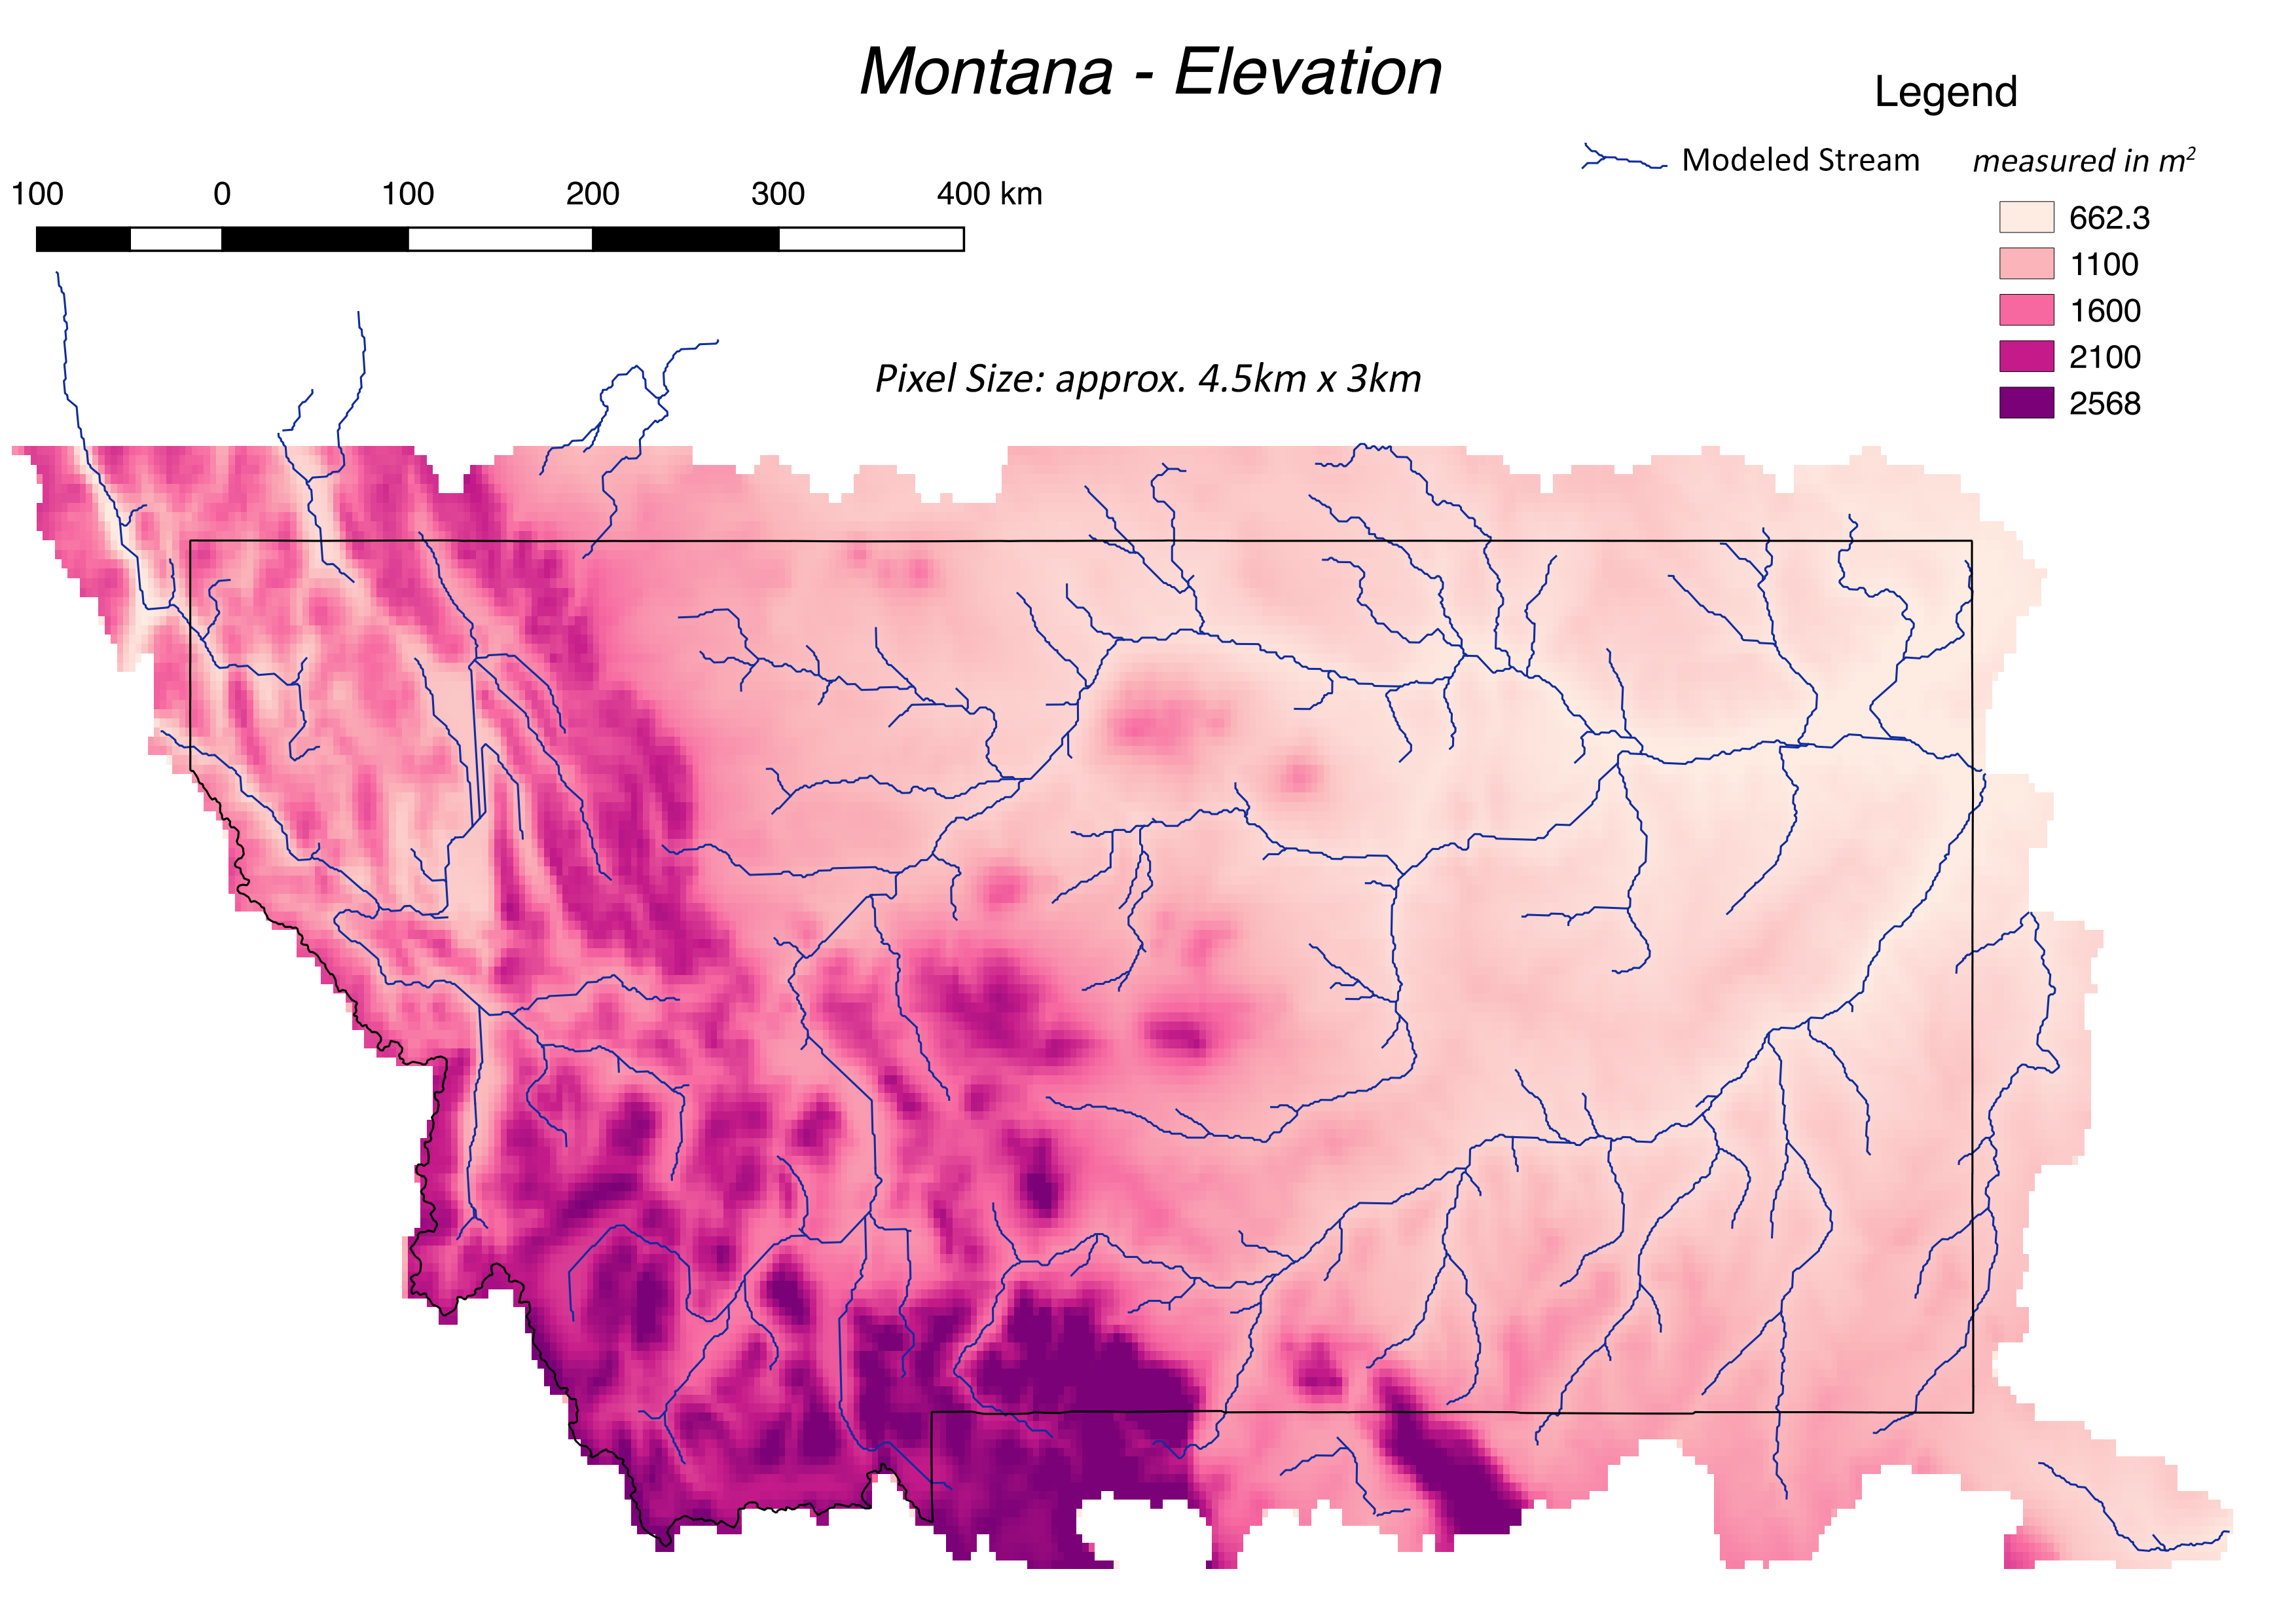
\includegraphics[width=0.95\textwidth]{elevation}
    \caption{Elevation throughout Montana}
    \label{fig:elevation}
\end{figure}

\section{Observation Data}

A Kalman Filter relies on one or more observed states for correction. Accordingly, observations were obtained for streamflows across Montana and snowfall across Montana. For streamflow, USGS streamflow data was collected at 86 sites. Each observed site was paired with the closest simulated \textbf{daWUAPhydroengine} stream outlet within a 2.5 mile cutoff. For snowfall, SNOWTEL sites monitored by the Natural Resources Conservation Service (NRCS) were used. 90 stations were chosen and matched to specific pixels in \textbf{daWUAPhydroengine}'s raster files.


\begin{table}[]
\caption{Observations} 
\begin{tabular}{lll}
Observed State ($x$) & Source                              & Dimensions  \\ \hline
streamflow  & USGS & 82   \\
swe         & NRCS & 90
\end{tabular}
\label{tab:obs}
\end{table}

\begin{figure}[h]
    \centering
    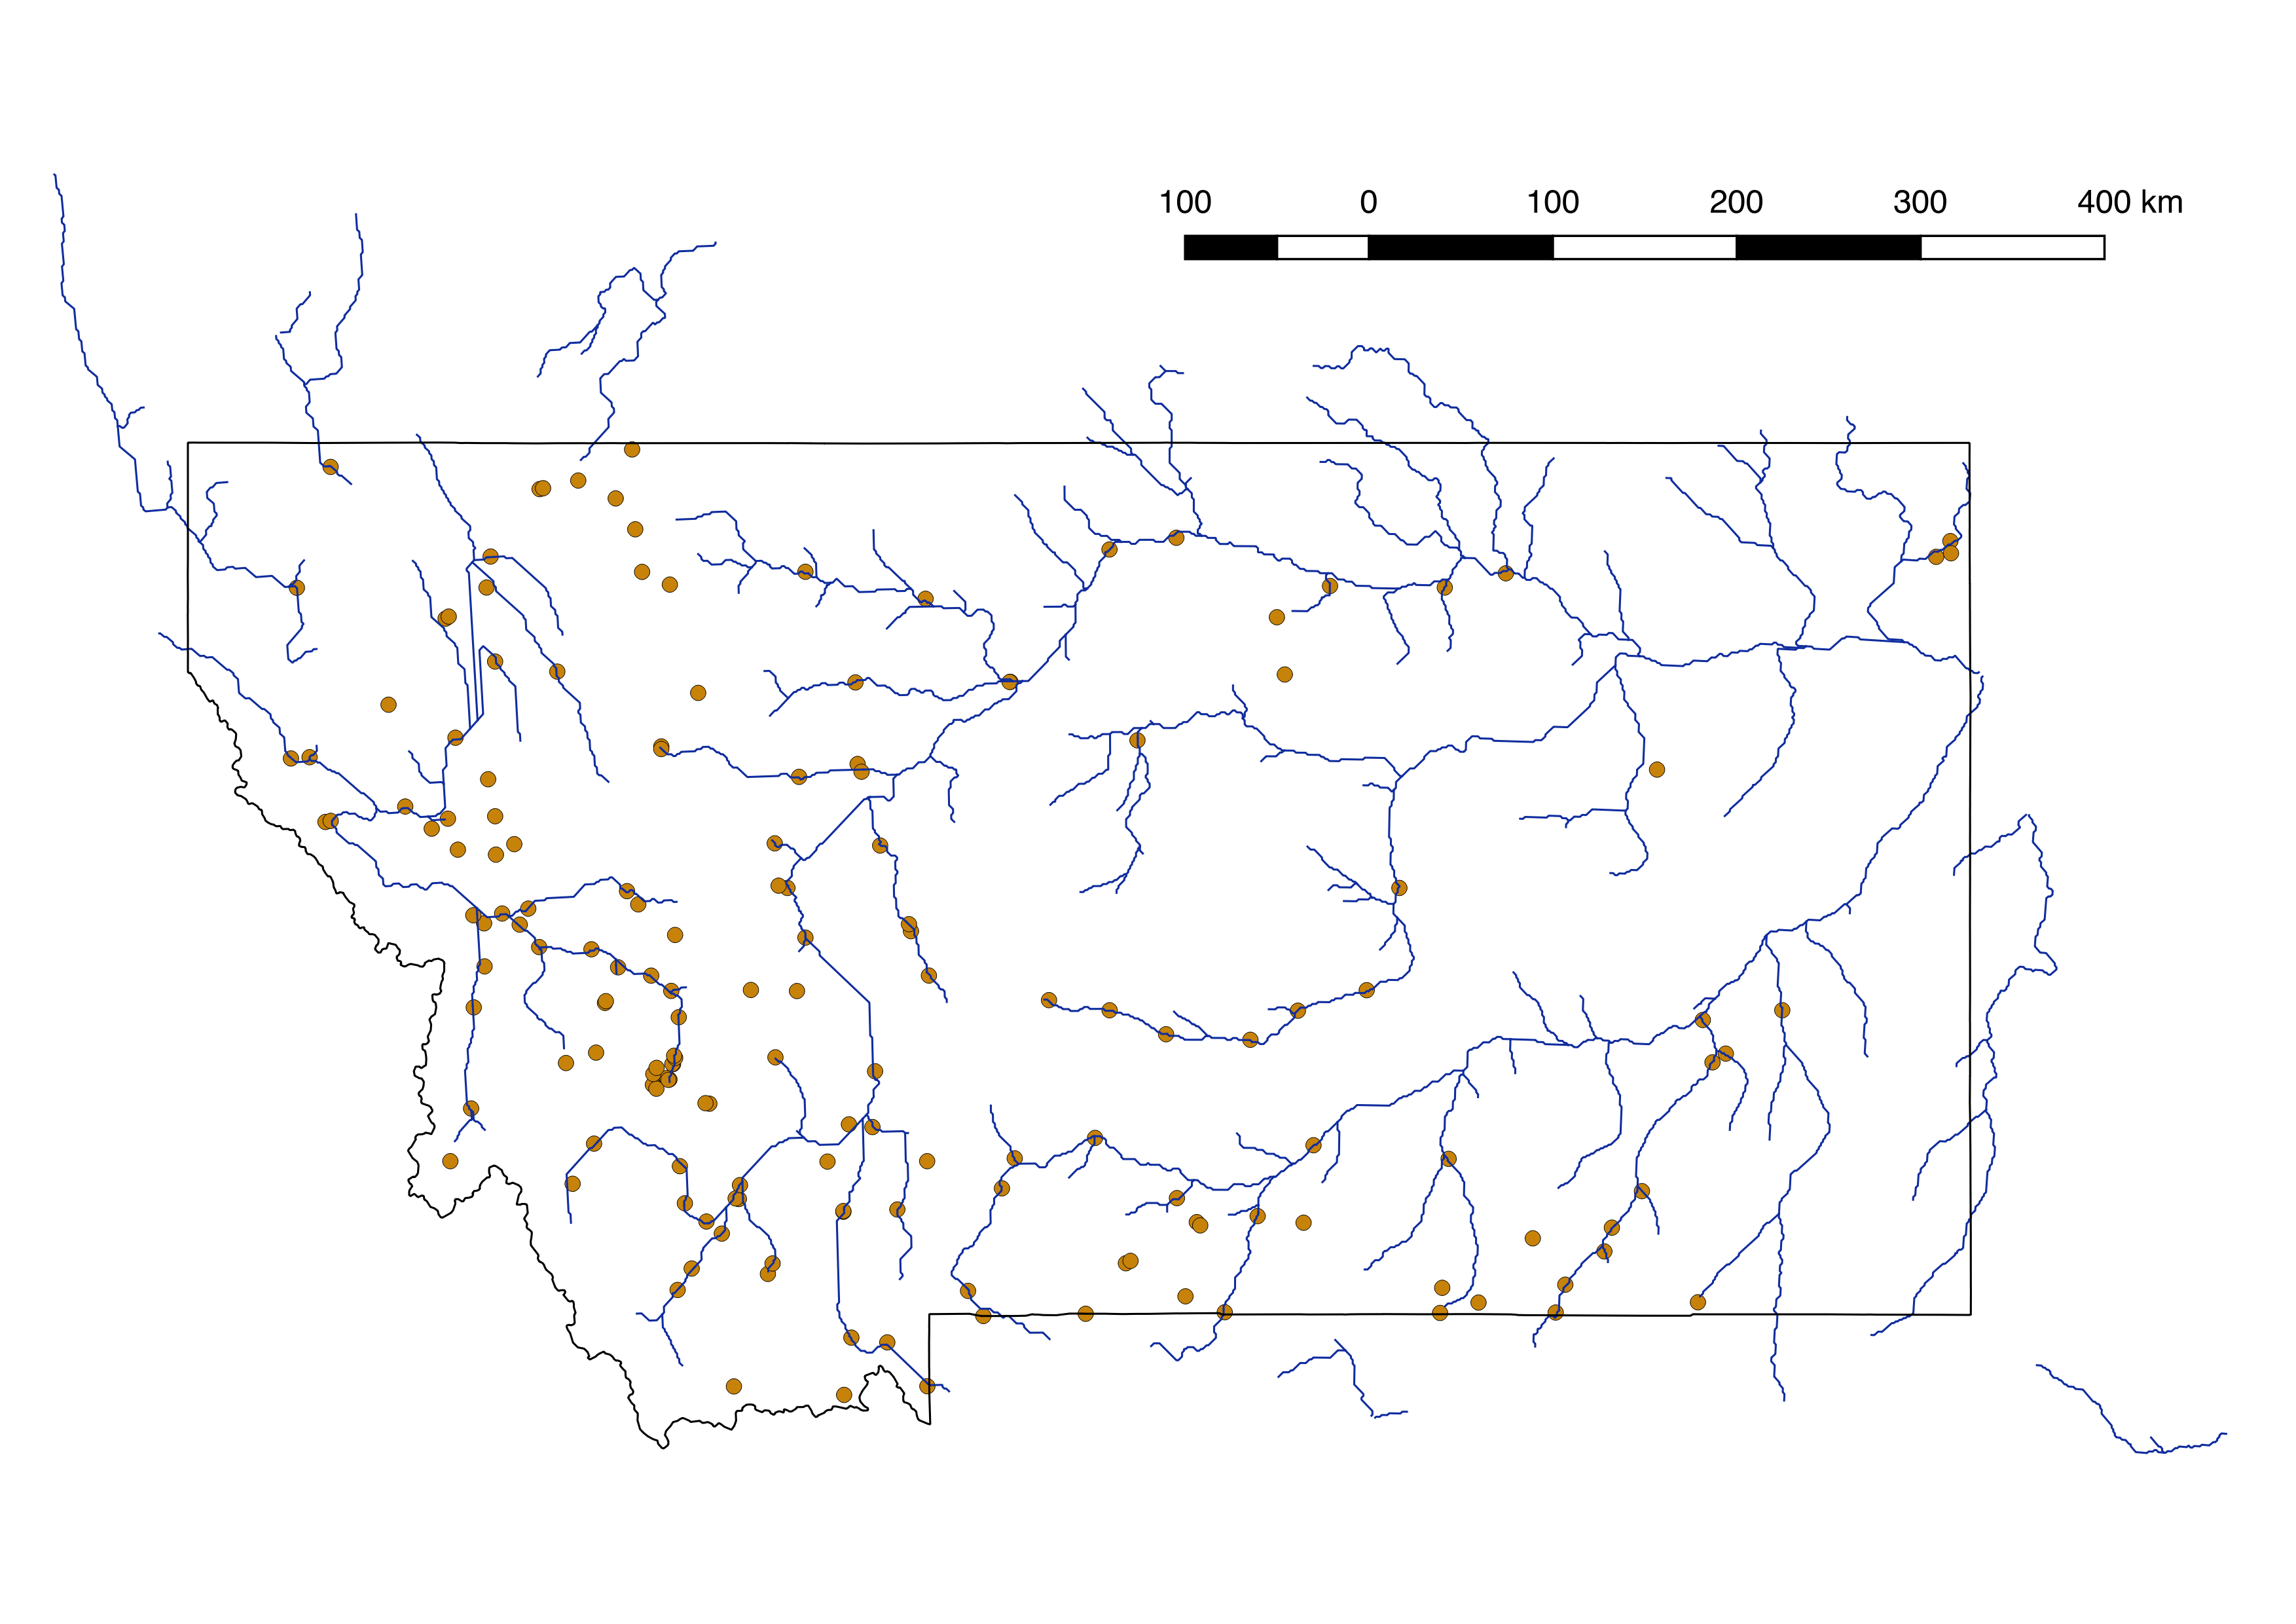
\includegraphics[width=0.95\textwidth]{stations}
    \caption{all SWE stations plotted against modeled streamflows}
    \label{fig:stations}
\end{figure}
%% This is an example first chapter.  You should put chapter/appendix that you
%% write into a separate file, and add a line \include{yourfilename} to
%% main.tex, where `yourfilename.tex' is the name of the chapter/appendix file.
%% You can process specific files by typing their names in at the 
%% \files=
%% prompt when you run the file main.tex through LaTeX.
\chapter{Example}

Micro-optimization is a technique to reduce the overall operation count of
floating point operations.  In a standard floating point unit, floating
point operations are fairly high level, such as ``multiply'' and ``add'';
in a micro floating point unit ($\mu$FPU), these have been broken down into
their constituent low-level floating point operations on the mantissas and
exponents of the floating point numbers.

Chapter two describes the architecture of the $\mu$FPU unit, and the
motivations for the design decisions made.

Chapter three describes the design of the compiler, as well as how the
optimizations discussed in section~\ref{ch1:opts} were implemented.

Chapter four describes the purpose of test code that was compiled, and which
statistics were gathered by running it through the simulator.  The purpose
is to measure what effect the micro-optimizations had, compared to
unoptimized code.  Possible future expansions to the project are also
discussed.

\section{Motivations for micro-optimization}

The idea of micro-optimization is motivated by the recent trends in computer
architecture towards low-level parallelism and small, pipelineable
instruction sets \cite{patterson:risc,rad83}.  By getting rid of more
complex instructions and concentrating on optimizing frequently used
instructions, substantial increases in performance were realized.

Another important motivation was the trend towards placing more of the
burden of performance on the compiler.  Many of the new architectures depend
on an intelligent, optimizing compiler in order to realize anywhere near
their peak performance
\cite{ellis:bulldog,pet87,coutant:precision-compilers}.  In these cases, the
compiler not only is responsible for faithfully generating native code to
match the source language, but also must be aware of instruction latencies,
delayed branches, pipeline stages, and a multitude of other factors in order
to generate fast code \cite{gib86}.

Taking these ideas one step further, it seems that the floating point
operations that are normally single, large instructions can be further broken
down into smaller, simpler, faster instructions, with more control in the
compiler and less in the hardware.  This is the idea behind a
micro-optimizing FPU; break the floating point instructions down into their
basic components and use a small, fast implementation, with a large part of
the burden of hardware allocation and optimization shifted towards
compile-time.

Along with the hardware speedups possible by using a $\mu$FPU, there are
also optimizations that the compiler can perform on the code that is
generated.  In a normal sequence of floating point operations, there are
many hidden redundancies that can be eliminated by allowing the compiler to
control the floating point operations down to their lowest level.  These
optimizations are described in detail in section~\ref{ch1:opts}.

\section{Description of micro-optimization}\label{ch1:opts}

In order to perform a sequence of floating point operations, a normal FPU
performs many redundant internal shifts and normalizations in the process of
performing a sequence of operations.  However, if a compiler can
decompose the floating point operations it needs down to the lowest level,
it then can optimize away many of these redundant operations.  

If there is some additional hardware support specifically for
micro-optimization, there are additional optimizations that can be
performed.  This hardware support entails extra ``guard bits'' on the
standard floating point formats, to allow several unnormalized operations to
be performed in a row without the loss information\footnote{A description of
the floating point format used is shown in figures~\ref{exponent-format}
and~\ref{mantissa-format}.}.  A discussion of the mathematics behind
unnormalized arithmetic is in appendix~\ref{unnorm-math}.

The optimizations that the compiler can perform fall into several categories:

\subsection{Post Multiply Normalization}

When more than two multiplications are performed in a row, the intermediate
normalization of the results between multiplications can be eliminated.
This is because with each multiplication, the mantissa can become
denormalized by at most one bit.  If there are guard bits on the mantissas
to prevent bits from ``falling off'' the end during multiplications, the
normalization can be postponed until after a sequence of several
multiplies\footnote{Using unnormalized numbers for math is not a new idea; a
good example of it is the Control Data CDC 6600, designed by Seymour Cray.
\cite{thornton:cdc6600} The CDC 6600 had all of its instructions performing
unnormalized arithmetic, with a separate {\tt NORMALIZE} instruction.}.

% This is an example of how you would use tgrind to include an example
% of source code; it is commented out in this template since the code
% example file does not exist.  To use it, you need to remove the '%' on the
% beginning of the line, and insert your own information in the call.
%
%\tagrind[htbp]{code/pmn.s.tex}{Post Multiply Normalization}{opt:pmn}

As you can see, the intermediate results can be multiplied together, with no
need for intermediate normalizations due to the guard bit.  It is only at
the end of the operation that the normalization must be performed, in order
to get it into a format suitable for storing in memory\footnote{Note that
for purposed of clarity, the pipeline delays were considered to be 0, and
the branches were not delayed.}.

\subsection{Block Exponent}

In a unoptimized sequence of additions, the sequence of operations is as
follows for each pair of numbers ($m_1$,$e_1$) and ($m_2$,$e_2$).
\begin{enumerate}
  \item Compare $e_1$ and $e_2$.
  \item Shift the mantissa associated with the smaller exponent $|e_1-e_2|$
        places to the right.
  \item Add $m_1$ and $m_2$.
  \item Find the first one in the resulting mantissa.
  \item Shift the resulting mantissa so that normalized
  \item Adjust the exponent accordingly.
\end{enumerate}

Out of 6 steps, only one is the actual addition, and the rest are involved
in aligning the mantissas prior to the add, and then normalizing the result
afterward.  In the block exponent optimization, the largest mantissa is
found to start with, and all the mantissa's shifted before any additions
take place.  Once the mantissas have been shifted, the additions can take
place one after another\footnote{This requires that for n consecutive
additions, there are $\log_{2}n$ high guard bits to prevent overflow.  In
the $\mu$FPU, there are 3 guard bits, making up to 8 consecutive additions
possible.}.  An example of the Block Exponent optimization on the expression
X = A + B + C is given in figure~\ref{opt:be}.

% This is an example of how you would use tgrind to include an example
% of source code; it is commented out in this template since the code
% example file does not exist.  To use it, you need to remove the '%' on the
% beginning of the line, and insert your own information in the call.
%
%\tgrind[htbp]{code/be.s.tex}{Block Exponent}{opt:be}

\section{Integer optimizations}

As well as the floating point optimizations described above, there are
also integer optimizations that can be used in the $\mu$FPU.  In concert
with the floating point optimizations, these can provide a significant
speedup.  

\subsection{Conversion to fixed point}

Integer operations are much faster than floating point operations; if it is
possible to replace floating point operations with fixed point operations,
this would provide a significant increase in speed.

This conversion can either take place automatically or or based on a
specific request from the programmer.  To do this automatically, the
compiler must either be very smart, or play fast and loose with the accuracy
and precision of the programmer's variables.  To be ``smart'', the computer
must track the ranges of all the floating point variables through the
program, and then see if there are any potential candidates for conversion
to floating point.  This technique is discussed further in
section~\ref{range-tracking}, where it was implemented.

The other way to do this is to rely on specific hints from the programmer
that a certain value will only assume a specific range, and that only a
specific precision is desired.  This is somewhat more taxing on the
programmer, in that he has to know the ranges that his values will take at
declaration time (something normally abstracted away), but it does provide
the opportunity for fine-tuning already working code.

Potential applications of this would be simulation programs, where the
variable represents some physical quantity; the constraints of the physical
system may provide bounds on the range the variable can take.
\subsection{Small Constant Multiplications}

One other class of optimizations that can be done is to replace
multiplications by small integer constants into some combination of
additions and shifts.  Addition and shifting can be significantly faster
than multiplication.  This is done by using some combination of
\begin{eqnarray*}
a_i & = & a_j + a_k \\
a_i & = & 2a_j + a_k \\
a_i & = & 4a_j + a_k \\
a_i & = & 8a_j + a_k \\
a_i & = & a_j - a_k \\
a_i & = & a_j \ll m \mbox{shift}
\end{eqnarray*}
instead of the multiplication.  For example, to multiply $s$ by 10 and store
the result in $r$, you could use:
\begin{eqnarray*}
r & = & 4s + s\\
r & = & r + r
\end{eqnarray*}
Or by 59:
\begin{eqnarray*}
t & = & 2s + s \\
r & = & 2t + s \\
r & = & 8r + t
\end{eqnarray*}
Similar combinations can be found for almost all of the smaller
integers\footnote{This optimization is only an ``optimization'', of course,
when the amount of time spent on the shifts and adds is less than the time
that would be spent doing the multiplication.  Since the time costs of these
operations are known to the compiler in order for it to do scheduling, it is
easy for the compiler to determine when this optimization is worth using.}.
\cite{magenheimer:precision}

\section{Other optimizations}

\subsection{Low-level parallelism}

The current trend is towards duplicating hardware at the lowest level to
provide parallelism\footnote{This can been seen in the i860; floating point
additions and multiplications can proceed at the same time, and the RISC
core be moving data in and out of the floating point registers and providing
flow control at the same time the floating point units are active. \cite{byte:i860}}

Conceptually, it is easy to take advantage to low-level parallelism in the
instruction stream by simply adding more functional units to the $\mu$FPU,
widening the instruction word to control them, and then scheduling as many
operations to take place at one time as possible.

However, simply adding more functional units can only be done so many times;
there is only a limited amount of parallelism directly available in the
instruction stream, and without it, much of the extra resources will go to
waste.  One process used to make more instructions potentially schedulable
at any given time is ``trace scheduling''.  This technique originated in the
Bulldog compiler for the original VLIW machine, the ELI-512.
\cite{ellis:bulldog,colwell:vliw}  In trace scheduling, code can be
scheduled through many basic blocks at one time, following a single
potential ``trace'' of program execution.  In this way, instructions that
{\em might\/} be executed depending on a conditional branch further down in
the instruction stream are scheduled, allowing an increase in the potential
parallelism.  To account for the cases where the expected branch wasn't
taken, correction code is inserted after the branches to undo the effects of
any prematurely executed instructions.

\subsection{Pipeline optimizations}

In addition to having operations going on in parallel across functional
units, it is also typical to have several operations in various stages of
completion in each unit.  This pipelining allows the throughput of the
functional units to be increased, with no increase in latency.

There are several ways pipelined operations can be optimized.  On the
hardware side, support can be added to allow data to be recirculated back
into the beginning of the pipeline from the end, saving a trip through the
registers.  On the software side, the compiler can utilize several tricks to
try to fill up as many of the pipeline delay slots as possible, as
seendescribed by Gibbons. \cite{gib86}



\appendix
\chapter{Tables}

\begin{table}
\caption{Armadillos}
\label{arm:table}
\begin{center}
\begin{tabular}{||l|l||}\hline
Armadillos & are \\\hline
our	   & friends \\\hline
\end{tabular}
\end{center}
\end{table}

\clearpage
\newpage

\chapter{Figures}

\vspace*{-3in}

\begin{figure}
\vspace{2.4in}
\caption{Armadillo slaying lawyer.}
\label{arm:fig1}
\end{figure}
\clearpage
\newpage

\begin{figure}
\vspace{2.4in}
\caption{Armadillo eradicating national debt.}
\label{arm:fig2}
\end{figure}
\clearpage
\newpage

%% This defines the bibliography file (main.bib) and the bibliography style.
%% If you want to create a bibliography file by hand, change the contents of
%% this file to a `thebibliography' environment.  For more information 
%% see section 4.3 of the LaTeX manual.
\begin{singlespace}
\bibliography{main}
\bibliographystyle{plain}
\end{singlespace}

\end{document}

